%!TEX program = xelatex
\documentclass[a4paper]{article}
\usepackage[preprint, nonatbib]{nips_2018}
\usepackage{float}

%\usepackage[UTF8]{ctex}

%\usepackage[square,numbers]{natbib}
%\bibliographystyle{abbrvnat}

\usepackage{amsmath}
\numberwithin{figure}{section}
\numberwithin{table}{section}
\usepackage[colorlinks,linkcolor=blue]{hyperref}
%\usepackage[utf8]{inputenc} % allow utf-8 input
\usepackage[T1]{fontenc}    % use 8-bit T1 fonts
\usepackage{hyperref}       % hyperlinks
\usepackage{url}            % simple URL typesetting
\usepackage{booktabs}       % professional-quality tables
\usepackage{amsfonts}       % blackboard math symbols
\usepackage{nicefrac}       % compact symbols for 1/2, etc.
\usepackage{microtype}      % microtypography
\usepackage{graphicx}
\usepackage{tabularx}
\usepackage{hyperref}
\usepackage{subfigure}
\usepackage{longtable}
\usepackage{cite}
\bibliographystyle{IEEEtran}
\title{Report for GEO1001 Homework 01}
\author{
	DONG Haoyang \\
	\texttt{5302501}
	\texttt{ }
	\texttt{H.Dong-2@student.tudelft.nl} \\

}

\begin{document}
\maketitle

\part{Introduction}

This is a report for GEO1001.2020 homework 01, the code files and other files can be find in: \href{https://github.com/HaoyangDong/GEO1001.2020--hw01}{HaoyangDong's Github Repository: GEO1001.2020--hw01} 

The dataset \cite{a} used in this work is posted on 24.08.2020 by Daniela Maiullari, Clara Garcia Sanchez.

\part{A1}

\section{A11}

\textbf{Question:}

Compute mean statistics (mean, variance and standard deviation for each of the sensors variables), what do you observe from the results?

\textbf{Answer:} 

Statistics can be found in Table\ref{TableA11}.

From the results, we can find the mean, variance, and standard deviation values of the measurement item like Temperature, Relative Humidity, and Global Temperature for all the sensors are similar, which may show that these sensors are set nearby and at similar altitude.Also, I found that the mean of Wind Speed of Sensor D is the highest.

\begin{longtable}{ccccc}
\label{Table: A1}

Measurement item & Device & Mean & Variance & Standard deviation\\
\hline
Wind Direction & A & 209.406 & 10104.858 & 100.523 \\
Wind Direction & B & 183.412 & 9973.188 & 99.866 \\
Wind Direction & C & 183.589 & 7700.249 & 87.751 \\
Wind Direction & D & 198.327 & 8130.602 & 90.17 \\
Wind Direction & E & 223.956 & 9304.524 & 96.46 \\
Wind Speed & A & 1.29 & 1.251 & 1.118 \\
Wind Speed & B & 1.242 & 1.301 & 1.141 \\
Wind Speed & C & 1.371 & 1.43 & 1.196 \\
Wind Speed & D & 1.582 & 1.739 & 1.319 \\
Wind Speed & E & 0.596 & 0.511 & 0.715 \\
Crosswind Speed & A & 0.965 & 0.926 & 0.962 \\
Crosswind Speed & B & 0.836 & 0.878 & 0.937 \\
Crosswind Speed & C & 0.963 & 1.042 & 1.021 \\
Crosswind Speed & D & 1.211 & 1.451 & 1.205 \\
Crosswind Speed & E & 0.439 & 0.316 & 0.562 \\
Headwind Speed & A & 0.164 & 1.035 & 1.017 \\
Headwind Speed & B & -0.13 & 1.256 & 1.121 \\
Headwind Speed & C & -0.263 & 1.271 & 1.127 \\
Headwind Speed & D & -0.301 & 1.232 & 1.11 \\
Headwind Speed & E & 0.195 & 0.319 & 0.565 \\
Temperature & A & 17.969 & 15.858 & 3.982 \\
Temperature & B & 18.065 & 16.622 & 4.077 \\
Temperature & C & 17.913 & 16.098 & 4.012 \\
Temperature & D & 17.996 & 16.099 & 4.012 \\
Temperature & E & 18.354 & 19.035 & 4.363 \\
Globe Temperature & A & 21.545 & 68.164 & 8.256 \\
Globe Temperature & B & 21.799 & 66.023 & 8.125 \\
Globe Temperature & C & 21.587 & 67.914 & 8.241 \\
Globe Temperature & D & 21.359 & 61.178 & 7.822 \\
Globe Temperature & E & 21.176 & 63.19 & 7.949 \\
Wind Chill & A & 17.838 & 16.258 & 4.032 \\
Wind Chill & B & 17.946 & 17.029 & 4.127 \\
Wind Chill & C & 17.773 & 16.534 & 4.066 \\
Wind Chill & D & 17.835 & 16.55 & 4.068 \\
Wind Chill & E & 18.294 & 19.129 & 4.374 \\
Relative Humidity & A & 78.185 & 375.858 & 19.387 \\
Relative Humidity & B & 77.878 & 408.458 & 20.21 \\
Relative Humidity & C & 77.963 & 374.471 & 19.351 \\
Relative Humidity & D & 77.942 & 389.698 & 19.741 \\
Relative Humidity & E & 76.793 & 406.33 & 20.158 \\
Heat Stress Index & A & 17.9 & 14.991 & 3.872 \\
Heat Stress Index & B & 18.004 & 15.433 & 3.928 \\
Heat Stress Index & C & 17.828 & 15.35 & 3.918 \\
Heat Stress Index & D & 17.922 & 15.112 & 3.887 \\
Heat Stress Index & E & 18.286 & 18.468 & 4.297 \\
Dew Point & A & 13.554 & 9.72 & 3.118 \\
Dew Point & B & 13.531 & 9.633 & 3.104 \\
Dew Point & C & 13.458 & 10.08 & 3.175 \\
Dew Point & D & 13.509 & 10.068 & 3.173 \\
Dew Point & E & 13.559 & 9.419 & 3.069 \\
Psychro Wet Bulb Temperature & A & 15.271 & 6.941 & 2.635 \\
Psychro Wet Bulb Temperature & B & 15.296 & 6.768 & 2.601 \\
Psychro Wet Bulb Temperature & C & 15.197 & 7.236 & 2.69 \\
Psychro Wet Bulb Temperature & D & 15.26 & 7.042 & 2.654 \\
Psychro Wet Bulb Temperature & E & 15.407 & 6.995 & 2.645 \\
Station Pressure & A & 1016.168 & 38.456 & 6.201 \\
Station Pressure & B & 1016.657 & 36.827 & 6.069 \\
Station Pressure & C & 1016.689 & 37.676 & 6.138 \\
Station Pressure & D & 1016.728 & 34.974 & 5.914 \\
Station Pressure & E & 1016.166 & 38.924 & 6.239 \\
Barometric Pressure & A & 1016.128 & 38.452 & 6.201 \\
Barometric Pressure & B & 1016.616 & 36.814 & 6.067 \\
Barometric Pressure & C & 1016.652 & 37.66 & 6.137 \\
Barometric Pressure & D & 1016.689 & 34.938 & 5.911 \\
Barometric Pressure & E & 1016.128 & 38.919 & 6.239 \\
Altitude & A & -25.987 & 2662.565 & 51.6 \\
Altitude & B & -30.058 & 2544.68 & 50.445 \\
Altitude & C & -30.339 & 2607.48 & 51.063 \\
Altitude & D & -30.653 & 2418.746 & 49.181 \\
Altitude & E & -25.961 & 2691.266 & 51.877 \\
Density Altitude & A & 137.317 & 26499.338 & 162.786 \\
Density Altitude & B & 135.581 & 26852.461 & 163.867 \\
Density Altitude & C & 129.623 & 26975.695 & 164.243 \\
Density Altitude & D & 132.411 & 26505.408 & 162.805 \\
Density Altitude & E & 150.84 & 29702.921 & 172.345 \\
NA Wet Bulb Temperature & A & 15.982 & 10.008 & 3.164 \\
NA Wet Bulb Temperature & B & 15.997 & 9.805 & 3.131 \\
NA Wet Bulb Temperature & C & 15.934 & 10.476 & 3.237 \\
NA Wet Bulb Temperature & D & 15.916 & 9.983 & 3.16 \\
NA Wet Bulb Temperature & E & 15.937 & 9.428 & 3.071 \\
WBGT & A & 17.254 & 16.129 & 4.016 \\
WBGT & B & 17.322 & 15.829 & 3.979 \\
WBGT & C & 17.225 & 16.54 & 4.067 \\
WBGT & D & 17.177 & 15.501 & 3.937 \\
WBGT & E & 17.186 & 15.484 & 3.935 \\
TWL  & A & 301.393 & 814.437 & 28.538 \\
TWL  & B & 299.452 & 789.75 & 28.102 \\
TWL  & C & 301.9 & 766.224 & 27.681 \\
TWL  & D & 305.255 & 615.761 & 24.815 \\
TWL  & E & 284.115 & 1289.392 & 35.908 \\
Direction Mag & A & 208.905 & 10101.596 & 100.507 \\
Direction Mag & B & 183.217 & 9971.418 & 99.857 \\
Direction Mag & C & 183.084 & 7701.506 & 87.758 \\
Direction Mag & D & 197.826 & 8132.027 & 90.178 \\
Direction Mag & E & 223.897 & 9264.263 & 96.251 \\
\hline
\caption{mean, variance and standard deviation for each of the sensors variables}
\label{TableA11}
\end{longtable}

\section{A12}

\textbf{Question:} 

Create 1 plot that contains histograms for the 5 sensors Temperature values. Compare histograms with 5 and 50 bins, why is the number of bins important?

\textbf{Answer:} 

The plots show in Figure \ref{Fig:A12}

The proper number of bins for a histogram is important. If the number of bins used is too small, the histogram cannot describe the data well. If there are have too many bins, the histogram will look like a broken comb, which will not give people a sense of distribution.

\begin{figure}
\centering
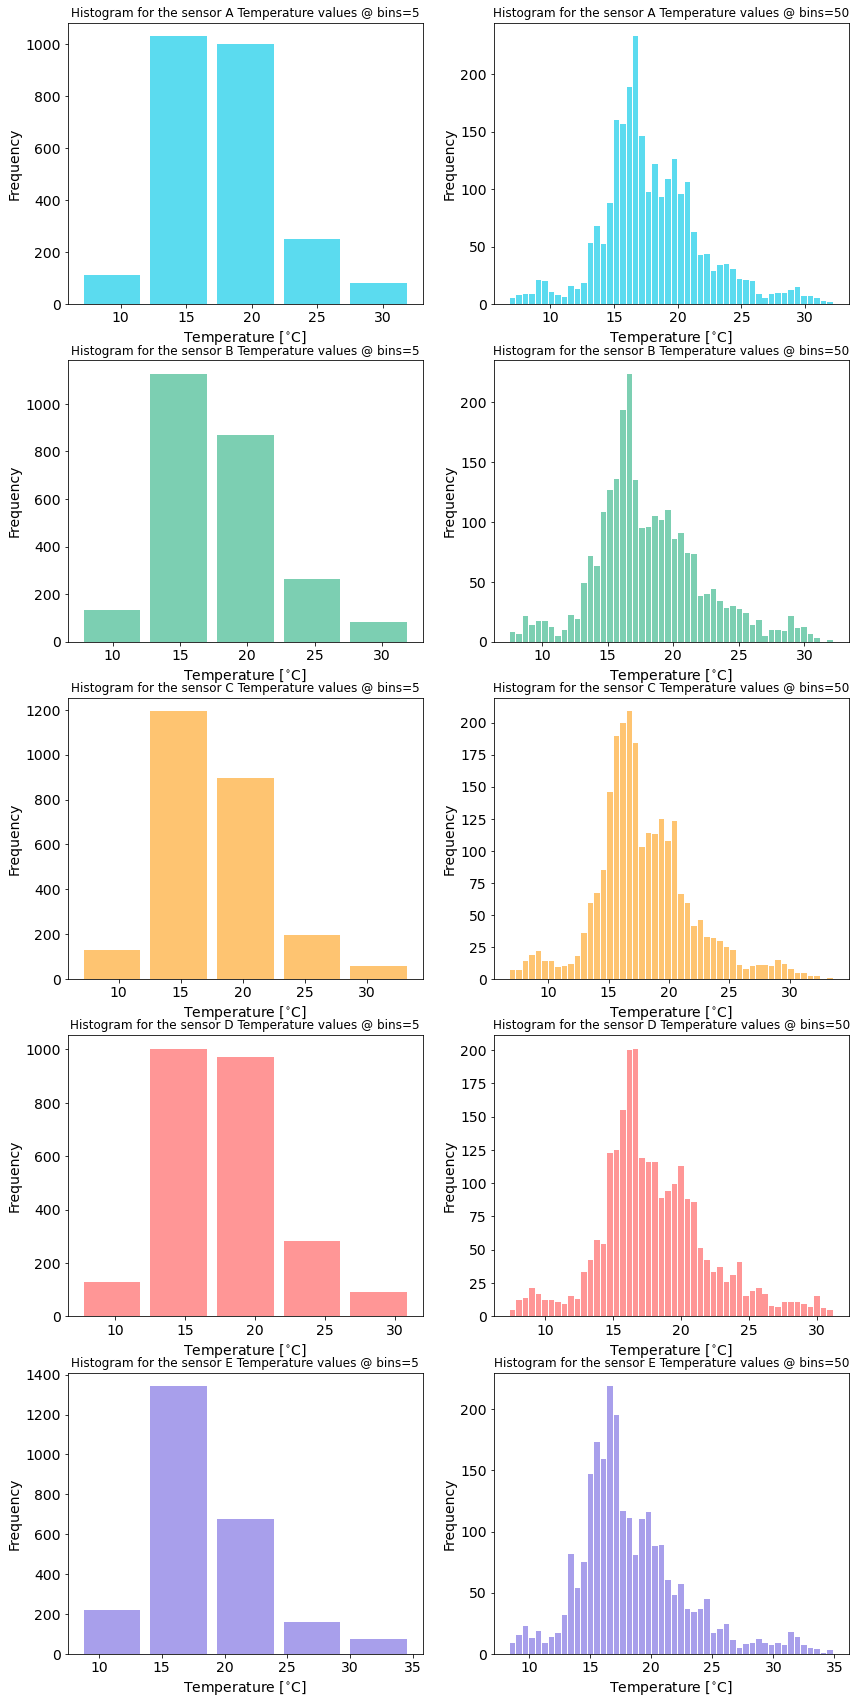
\includegraphics[scale=0.38]{Figures/figA12.png}
\caption{Histograms for the 5 sensors Temperature values. Compare histograms with 5 and 50 bins}

\label{Fig:A12}
\end{figure}
\section{A13}

\textbf{Question:}

Create 1 plot where frequency poligons for the 5 sensors Temperature values overlap in different colors with a legend.

\textbf{Answer:}

The plot shows in Figure \ref{Fig:A13}.

\begin{figure}
\centering
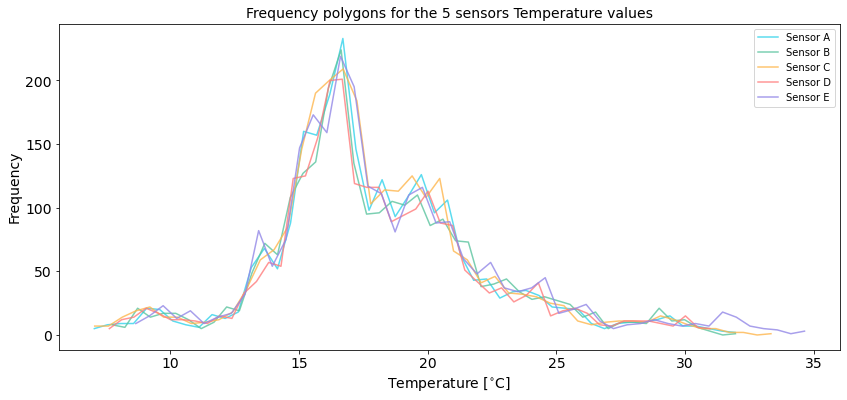
\includegraphics[scale=0.38]{Figures/figA13.png}
\caption{Frequency poligons for the 5 sensors Temperature values overlap in different colors with a legend}

\label{Fig:A13}
\end{figure}

\section{A14}

\textbf{Question:}

Generate 3 plots that include the 5 sensors boxplot for: Wind Speed, Wind Direction and Temperature.

\textbf{Answer:}

The plot shows in Figure \ref{Fig:A14}.

\begin{figure}
\centering
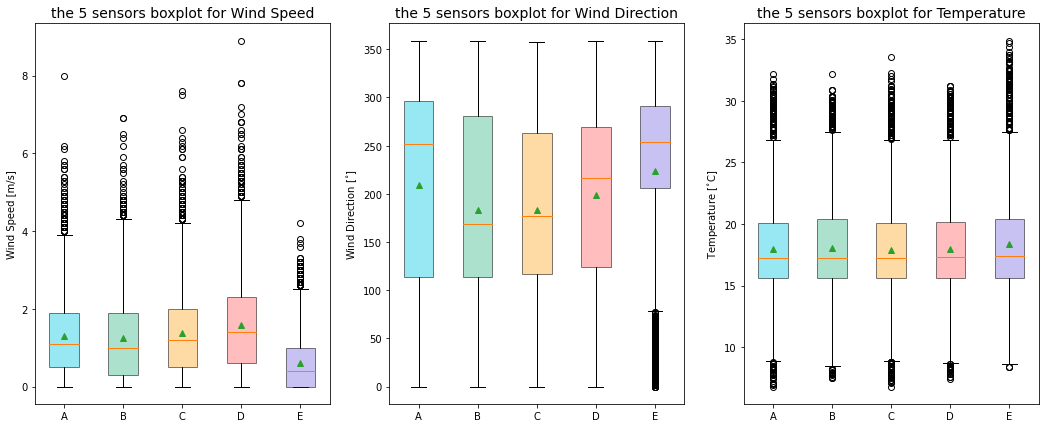
\includegraphics[scale=0.38]{Figures/figA14.png}
\caption{The 5 sensors boxplot for: Wind Speed, Wind Direction and Temperature}

\label{Fig:A14}
\end{figure}

\part{A2}

\section{A21}

\textbf{Question:}

Plot PMF, PDF and CDF for the 5 sensors Temperature values in independent plots (or subplots). Describe the behaviour of the distributions, are they all similar? what about their tails?

\textbf{Answer:}

The plot shows in Figure \ref{Fig:A21}.

Since the CDF, cumulative distribution function, maps from a value to its percentile rank, it looks quiet different from other plots. A PDF or KDE shows density rather than probability but a KDE discribes the Temperature values better than a normal PDF. Also the normal PDF has thinner tails than the PMF and KDE. The PMF and KDE look similar the main difference is that the y-axis of PMF means probability whille that of KDE means density.

\begin{figure}
\centering
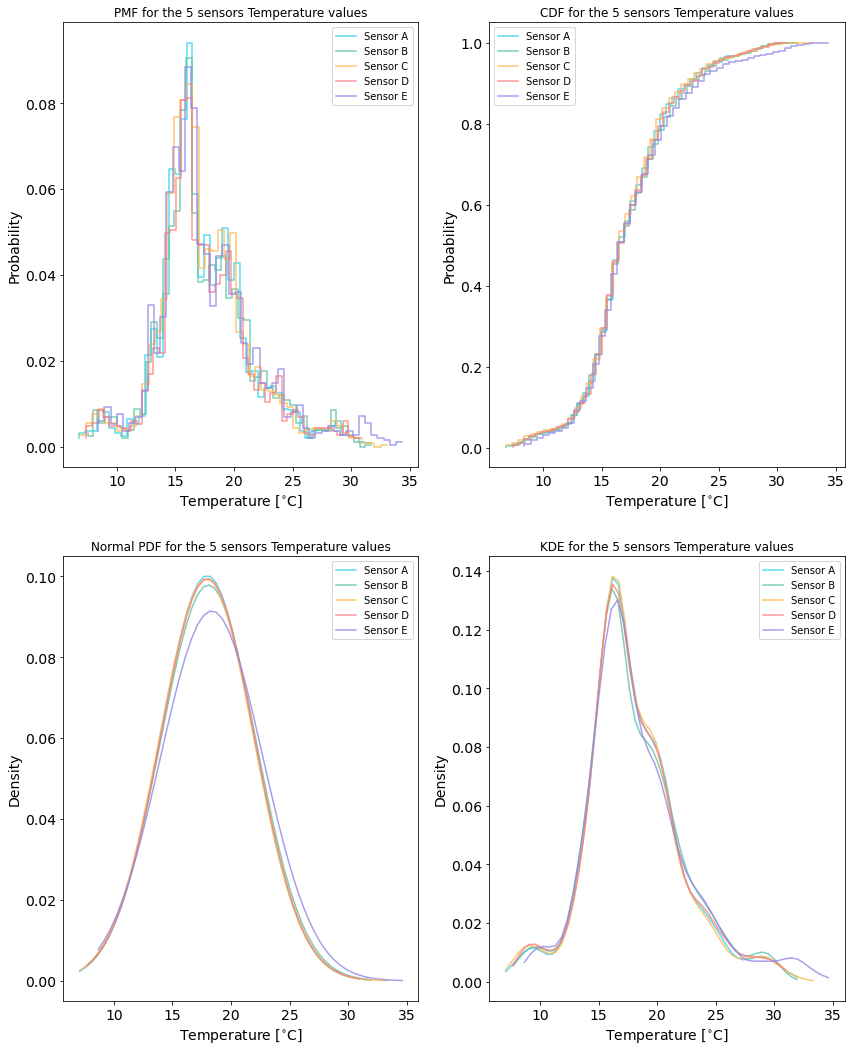
\includegraphics[scale=0.38]{Figures/figA21.png}
\caption{PMF, CDF, normal PDF, and KDE for the 5 sensors Temperature values}
\label{Fig:A21}
\end{figure}

\section{A22}

\textbf{Question:}

For the Wind Speed values, plot the pdf and the kernel density estimation. Comment the differences.

\textbf{Answer:}

The plot shows in Figure \ref{Fig:A22}.

A normal PDF in this case can not discribe the data very well. Meanwhile, the KDE shows more details and the skewness also shows more apparent in the KDE plot.

\begin{figure}
\centering
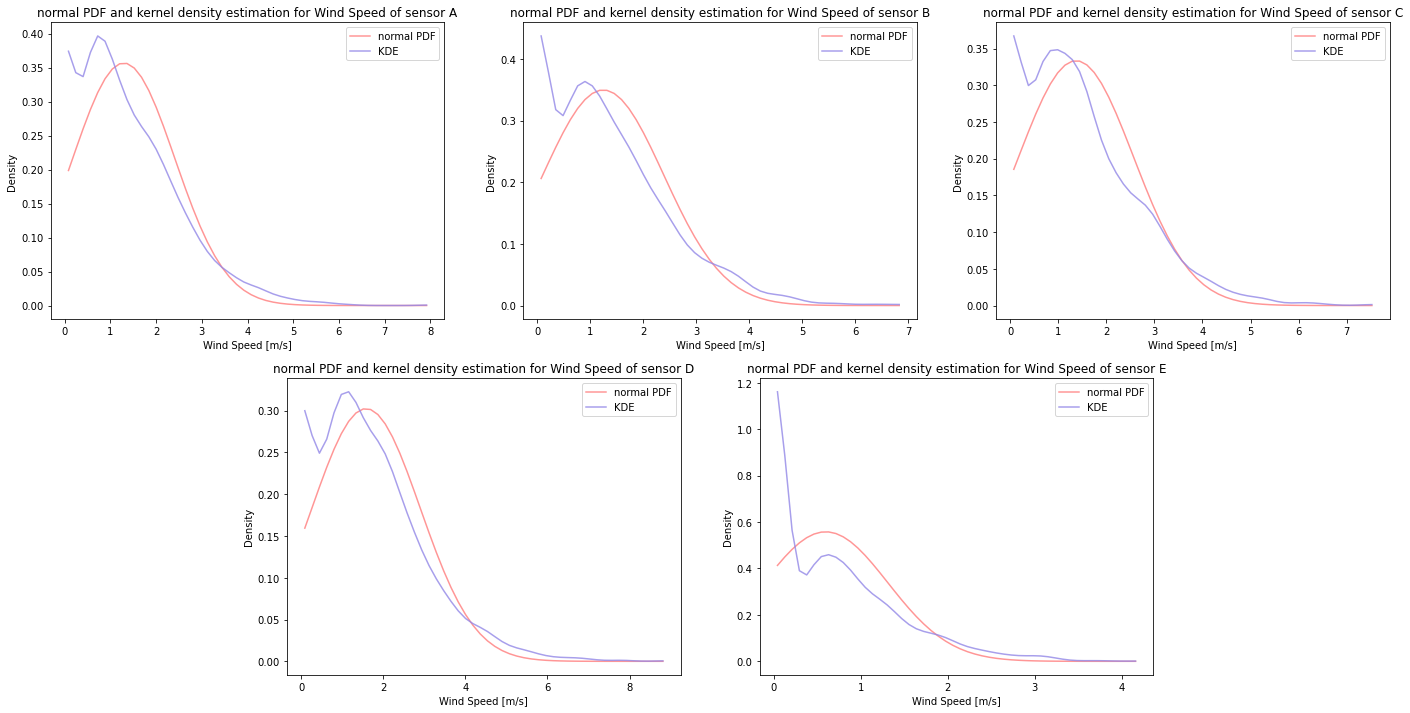
\includegraphics[scale=0.34]{Figures/figA22.png}
\caption{The normal PDF and the KDE for the Wind Speed}
\label{Fig:A22}
\end{figure}

\part{A3}

\section{A31}

\textbf{Question:}

Compute the correlations between all the sensors for the variables: Temperature, Wet Bulb Globe Temperature (WBGT), Crosswind Speed. Perform correlation between sensors with the same variable, not between two different variables; for example, correlate Temperature time series between sensor A and B. Use Pearson’s and Spearmann’s rank coefficients. Make a scatter plot with both coefficients with the 3 variables.

\textbf{Answer:}

The plot shows in Figure \ref{Fig:A31}.

\begin{figure}
\centering
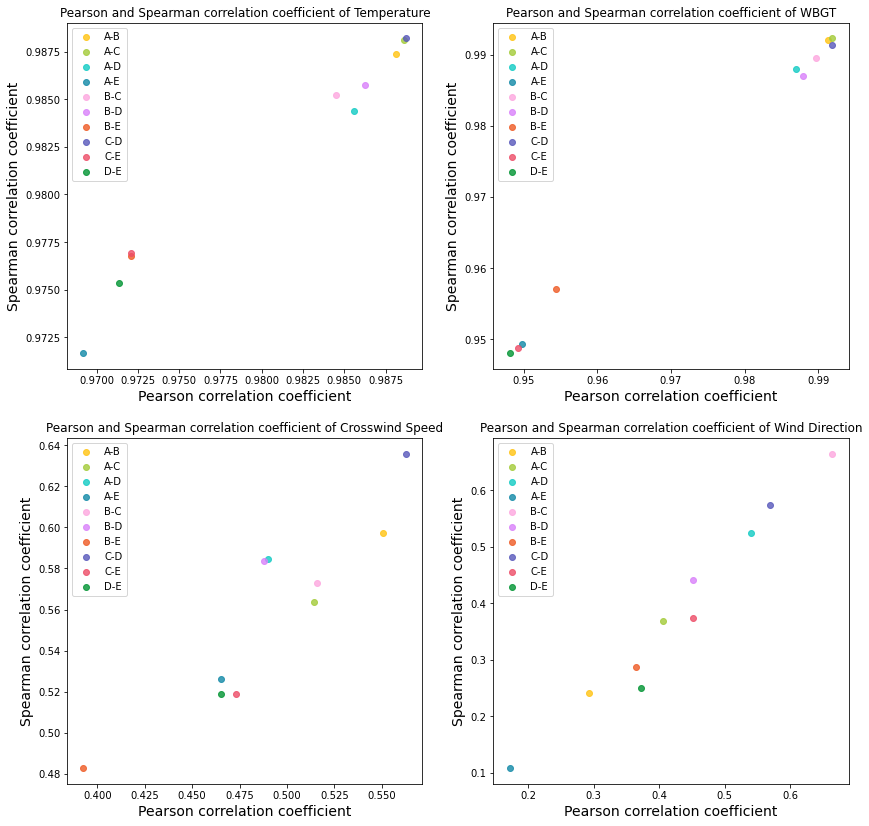
\includegraphics[scale=0.4]{Figures/figA31.png}
\caption{Scatter plots of Pearson’s and Spearmann’s rank coefficients between all the sensors}
\label{Fig:A31}
\end{figure}

\section{A32}

\textbf{Question:}

What can you say about the sensors’ correlations?

\textbf{Answer:}

In Figure \ref{Fig:A31}, we can find that, all the sensors show strong correlation in Temperature and WBGT and for the Crosswind Speed, the C and D show strong correlation but B and E show poor correlation. In fact, all the combinations of E show poor correlation in Crosswind Speed.

\section{A33}

\textbf{Question:}

If we told you that that the sensors are located as follows, hypothesize which location would you assign to each sensor and reason your hypothesis using the correlations.

\textbf{Answer:}

For all the combinations of E show poor correlation in Crosswind Speed and Wind Direction, E should be the most isolated one. C and D show strong correlations in both Crosswind Speed and Wind Direction. Meanwhile, B and C show strong correlations in Wind Direction, and A and E have almost zero correlations. 

So the location of each sensors should be like Figure \ref{Fig:A33}.



\begin{figure}
\centering
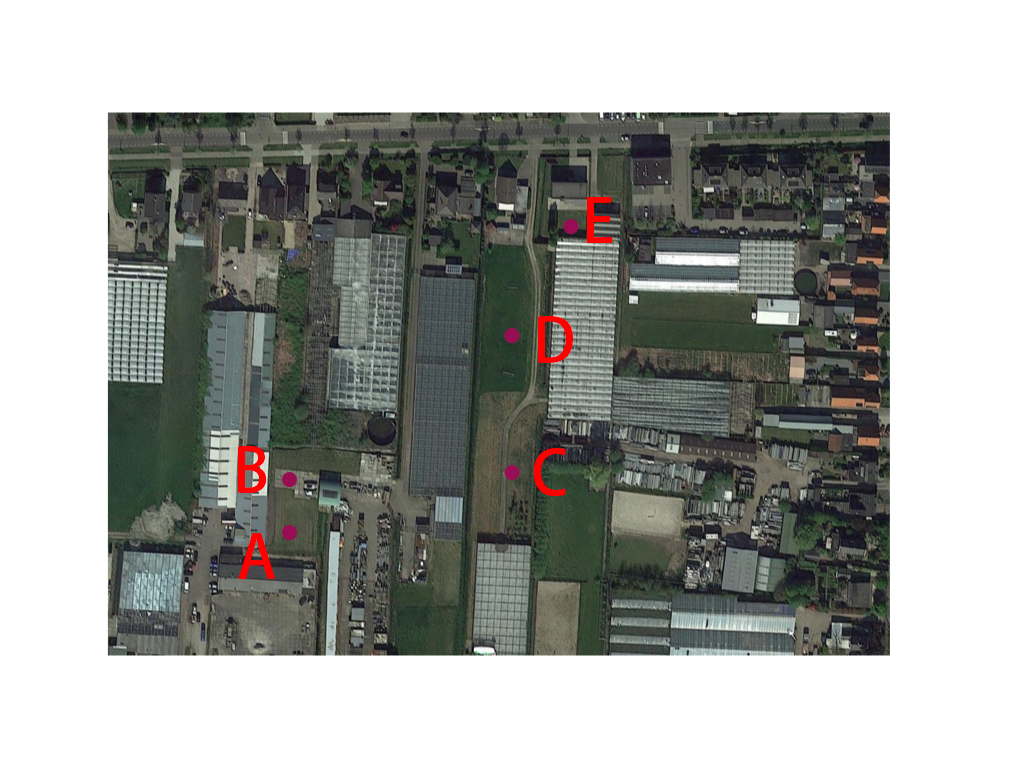
\includegraphics[scale=0.45]{Figures/figA33.jpg}
\caption{Locations of the sensors}
\label{Fig:A33}
\end{figure}


\part{A4}

\section{A41}

\textbf{Question:}

Plot the CDF for all the sensors and for variables Temperature and Wind Speed, then compute the 95\% confidence intervals for variables Temperature and Wind Speed for all the sensors and save them in a table (txt or csv form).

\textbf{Answer:}

The plot shows in Figure \ref{Fig:A41}. The csv form can be found in: \href{https://github.com/HaoyangDong/GEO1001.2020--hw01}{HaoyangDong's Github Repository: GEO1001.2020--hw01} 

\begin{figure}
\centering
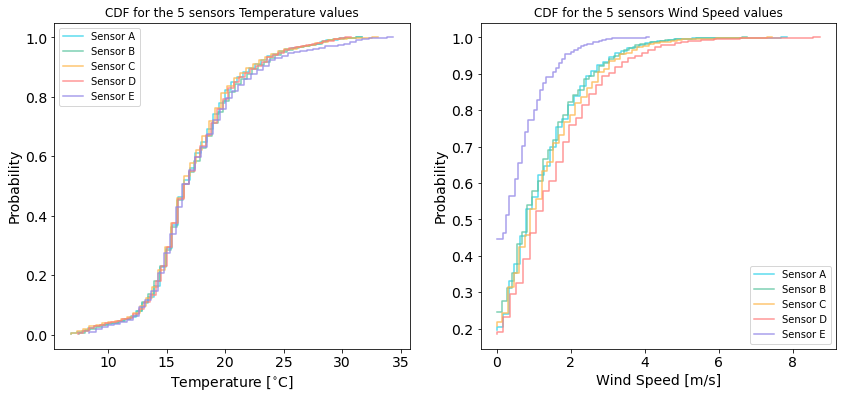
\includegraphics[scale=0.45]{Figures/figA41.png}
\caption{The CDF for all the sensors and for variables Temperature and Wind Speed}
\label{Fig:A41}
\end{figure}


\section{A42}

\textbf{Question:}

Test the hypothesis: the time series for Temperature and Wind Speed are the same for sensors:

1) E, D;

2) D, C;

3) C, B;

4) B, A.

\textbf{Answer:}

Temperature same hypothesis for E and D: Statistics=3.000, p=0.003 $\rightarrow$ Different distributions (reject H0)

Wind Speed same hypothesis for E and D: Statistics=-32.673, p=0.000 $\rightarrow$ Different distributions (reject H0)


Temperature same hypothesis for D and C: Statistics=0.729, p=0.466 $\rightarrow$ Same distributions (fail to reject H0)

Wind Speed same hypothesis for D and C: Statistics=5.871, p=0.000 $\rightarrow$ Different distributions (reject H0)


Temperature same hypothesis for C and B: Statistics=-1.324, p=0.185 $\rightarrow$ Same distributions (fail to reject H0)

Wind Speed same hypothesis for C and B: Statistics=3.893, p=0.000 $\rightarrow$ Different distributions (reject H0)


Temperature same hypothesis for B and A: Statistics=0.841, p=0.400 $\rightarrow$ Same distributions (fail to reject H0)

Wind Speed same hypothesis for B and A: Statistics=-1.501, p=0.134 $\rightarrow$ Same distributions (fail to reject H0)

\section{A42}

\textbf{Question:}

What could you conclude from the p-values?

\textbf{Answer:}

The time series for Temperature and Wind Speed are the same for sensors A and B. The time series for Temperature are the same for C and D and C and B. The time series for Temperature and Wind Speed are the different for sensors D and E.

\part{Bonus question}

\textbf{Question:}

Your “employer” wants to estimate the day of maximum and minimum potential energy consumption due to air conditioning usage. To hypothesize regarding those days, you are asked to identify the hottest and coolest day of the measurement time series provided. How would you do that? Reason and program the python rutine that would allow you to identify those days.

\textbf{Answer:}

By summing up the temperature values for all sensors in the same day and computering the mean temperature, then sort these mean values and find the min and max.

The hotest day: 2020/06/26

The coldest day: 2020/06/10

\bibliographystyle{plain}
\bibliography{Measured.bib}

\end{document}


